% Book pp. 63-67 (PDF pp. 64-68)
\section{Determining Maximum/Minimum Values}

In year one, we learnt how to solve linear equations and inequalities using graphing
and algebraic reasoning. With this knowledge, we will be able to graph polygons
when given specific linear equations or inequalities which will help us determine
the maximum/minimum value for a function.

Working in pairs or groups, go through this activity to review graphing of linear
inequalities.

\begin{activity}{Activity 2.3 -- Graphing Linear Inequalities}
\begin{enumerate}
  \item Pick a graph book/sheet
  \item Represent the following inequalities graphically
  \begin{enumerate}
    \item[a.] $y \le 0.67x + 2$
    \item[b.] $y \le -x + 2$
    \item[c.] $y \ge -2$
  \end{enumerate}
  \item Write out the coordinates for the points at which the inequalities intersect.
  \item What polygon did the intersecting lines create?
  \item Does your graph look like the one in Figure. 2.1: Graphing Linear
  Inequalities?
\end{enumerate}
\begin{center}
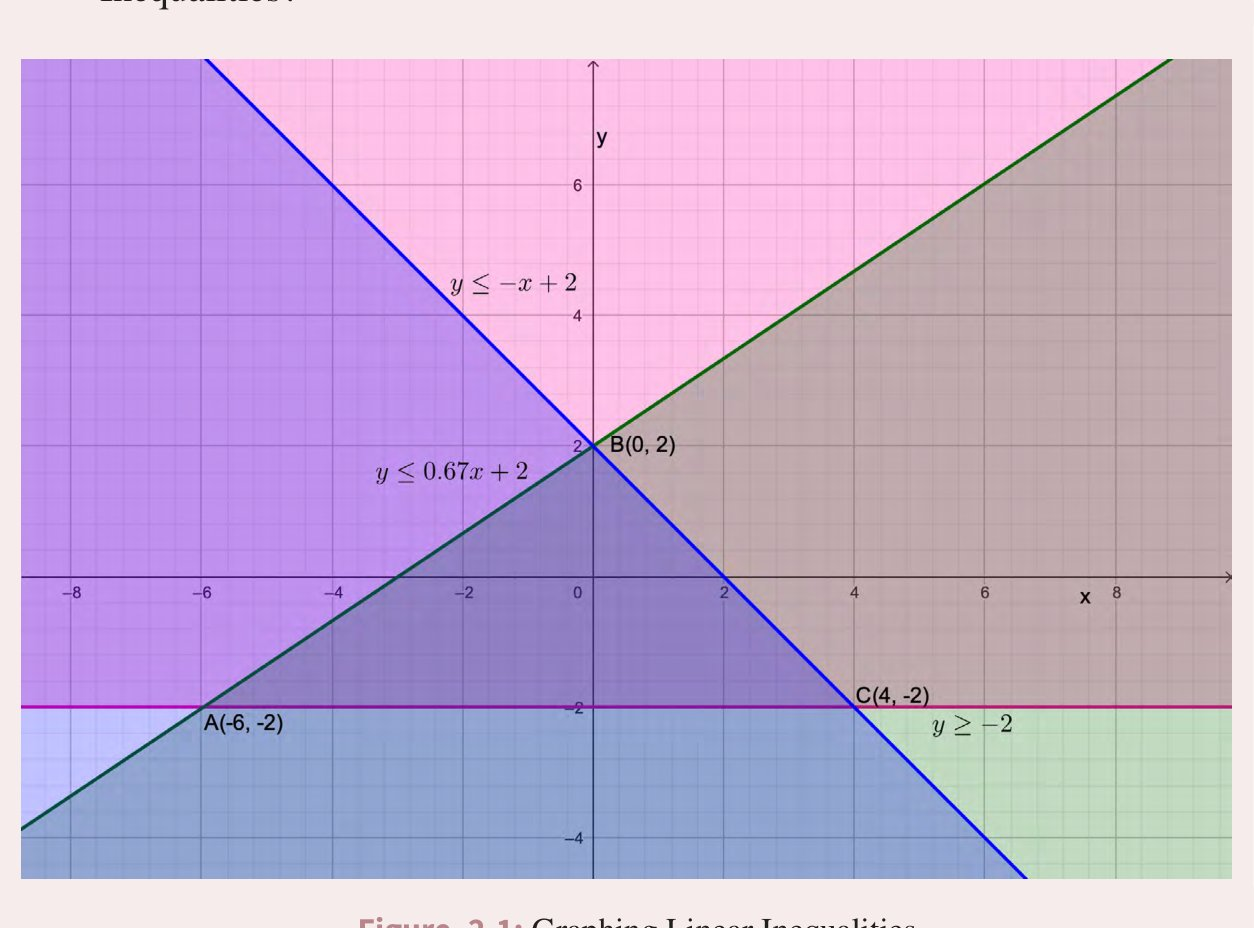
\includegraphics[width=0.85\linewidth]{figures/fig2-1.jpg}
\end{center}
\figcaption{2.1}{Graphing Linear Inequalities}
\end{activity}

Congratulations! You have adequately remembered how to graph linear
inequalities.

Now, we will learn how to determine the maximum/minimum value(s) of a given
function.

We can determine the maximum or minimum value of a given function based
on a specific objective. Maximum values are the highest points of a function
while minimum values are the lowest points of a function. In finding maximum
or minimum values of a function algebraically, you have to substitute all the
coordinates of the vertices of the region of interest that forms the solution to the
function. For example, if you are interested in getting the maximum/minimum
area of a given rectangle, you would evaluate the function at each corner or
edge by substituting the coordinates. If the polygon of interest (triangle, square,
etc.) is represented graphically, you need to identify the pair of coordinates and
substitute in the given function. On the other hand, if equations of lines are given,
you solve these equations simultaneously and determine the values for the pair of
coordinates.

\begin{example}{Example 2.13}
Evaluate the expression $V = 2x - 3y$ for the given feasible region to determine
the point at which `V' has a maximum value and the point at which `V' has a
minimum value.
\begin{center}
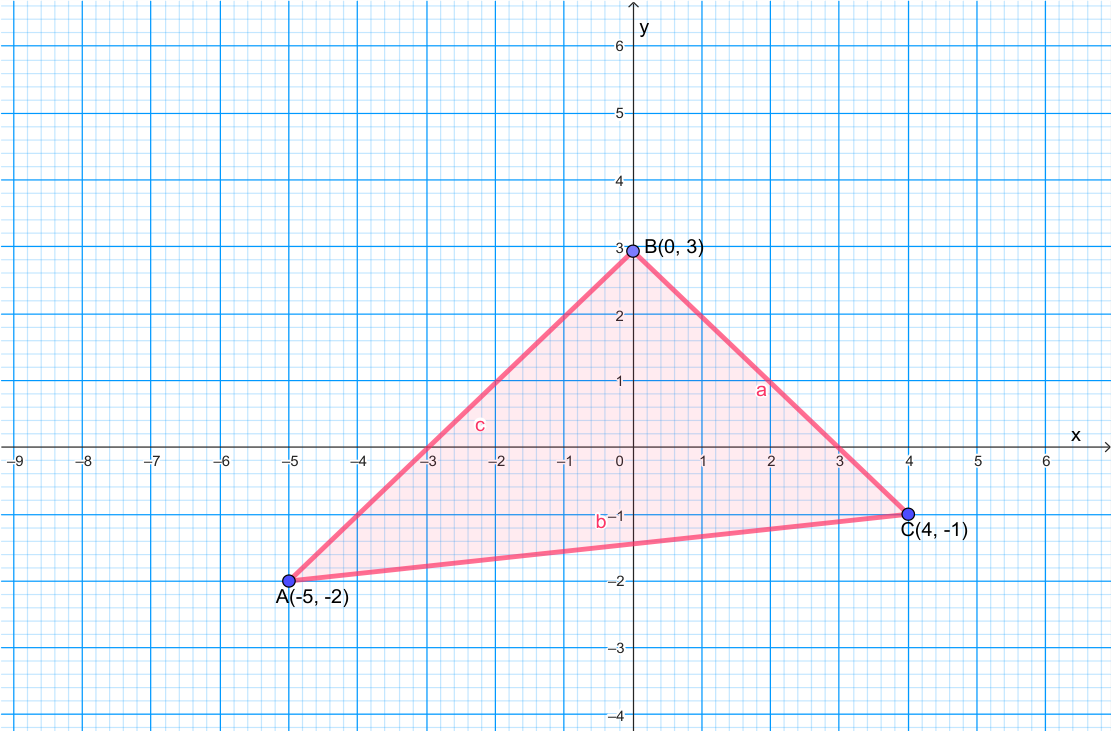
\includegraphics[width=0.8\linewidth]{figures/fig2-2.png}
\end{center}
% The book prints this graph without a caption; the solution calls it Figure 2.2.

\solution
\textbf{Step 1:} Identify all the vertices in Figure. 2.2

A $(-5, -2)$, B$(0, 3)$ and C $(4, -1)$

\textbf{Step 2:} Substitute the coordinates of each of the vertices in the function
$V = 2x - 3y$ and compute.

For $(-5, -2)$, $x = -5$, $y = -2$.
\begin{align*}
  V &= 2(-5) - 3(-2) \\
    &= -4
\end{align*}
For $(0, 3)$, $x = 0$, $y = 3$.
\begin{align*}
  V &= 2(0) - 3(3) \\
    &= -9
\end{align*}
For $(4, -1)$, $x = 4$, $y = -1$.
\begin{align*}
  V &= 2(4) - 3(-1) \\
    &= 11
\end{align*}

\textbf{Step 3:} Choose the highest result as the maximum value and the least as the
minimum value

Maximum value is 11 at vertex $(4, -1)$.

Minimum value is $-9$ at vertex $(0, 3)$.
\end{example}

\begin{example}{Example 2.14}
On the same graph, illustrate the inequalities, $y \ge \frac{7}{3}x - 5$, $y \le x - 1$ and
$x \ge 0$.

Using the polygon created, determine the minimum and maximum values of the
function $m = 7x - y$.

\solution
\textbf{Step 1:} Draw the three linear inequalities on a graph sheet.
\begin{center}
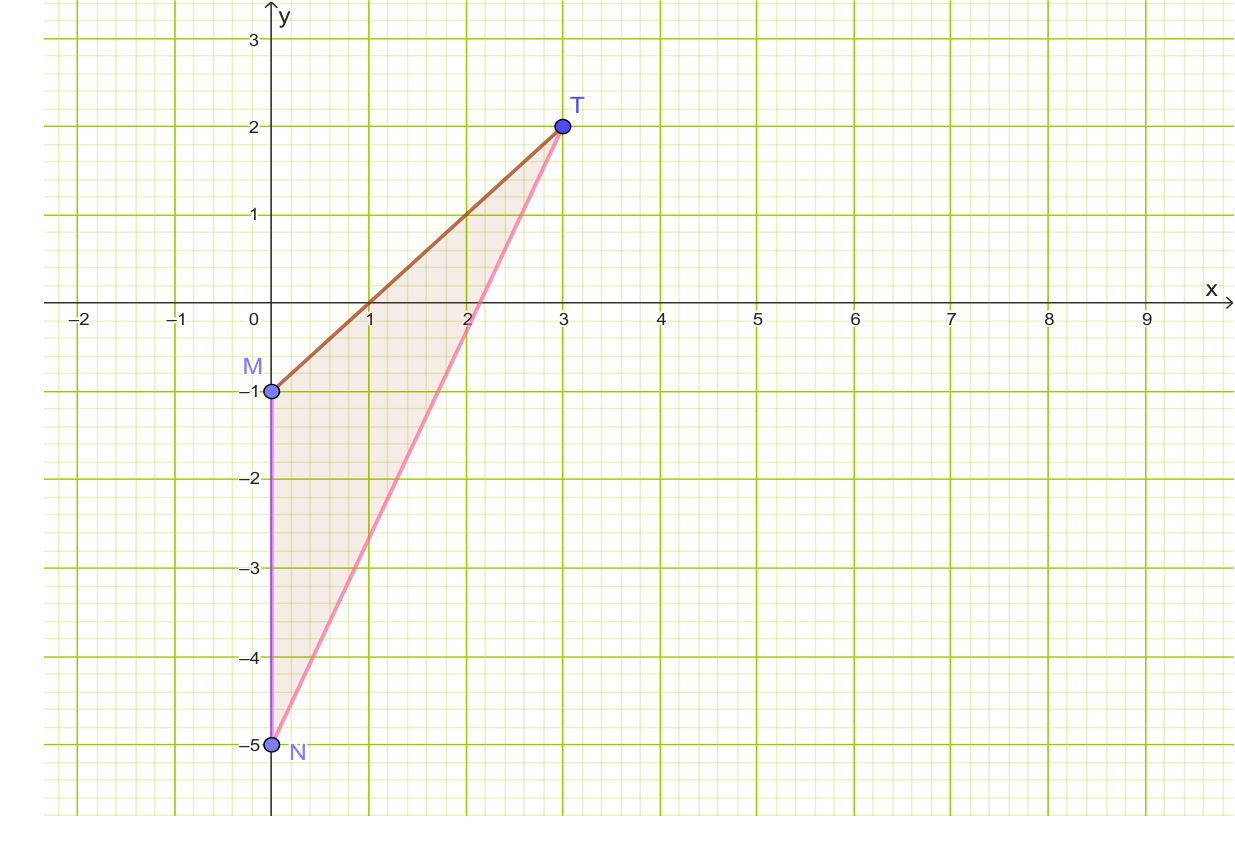
\includegraphics[width=0.85\linewidth]{figures/fig2-3.png}
\end{center}
\figcaption{2.3}{Graphical representation of inequalities in Example 2.14}

\textbf{Step 2:} Identify the coordinates of the vertices polygon created as a result of the
intersection of the lines.

M$(0, -1)$, T$(3, 2)$ and N$(0, -5)$

\textbf{Step 3:} Substitute the values of the coordinates in the function $m = 7x - y$.

For $(0, -1)$, $x = 0$, $y = -1$.
\begin{align*}
  m &= 7(0) - (-1) \\
    &= 1
\end{align*}
For $(3, 2)$, $x = 3$, $y = 2$.
\begin{align*}
  m &= 7(3) - 2 \\
    &= 19
\end{align*}
For $(0, -5)$, $x = 0$, $y = -5$.
\begin{align*}
  m &= 7(0) - (-5) \\
    &= 5
\end{align*}

\textbf{Step 4:} Select the highest result as the maximum value and the least as the
minimum value

Maximum value is 19 at vertex $(3, 2)$.

Minimum value is 1 at vertex $(0, -1)$.
\end{example}

\begin{example}{Example 2.15}
On the same graph, illustrate the inequalities, $x + y \le 8$, $y \ge 2$, $x - y \le 3$,
$-x + 2y \le 10$ and $x \ge 1$. Using the boundaries of the polygon created, determine the
minimum and maximum values of the function $w = x^2 + y^2$.

\solution
Step 1: Draw the five linear inequalities on a graph sheet.
\begin{center}
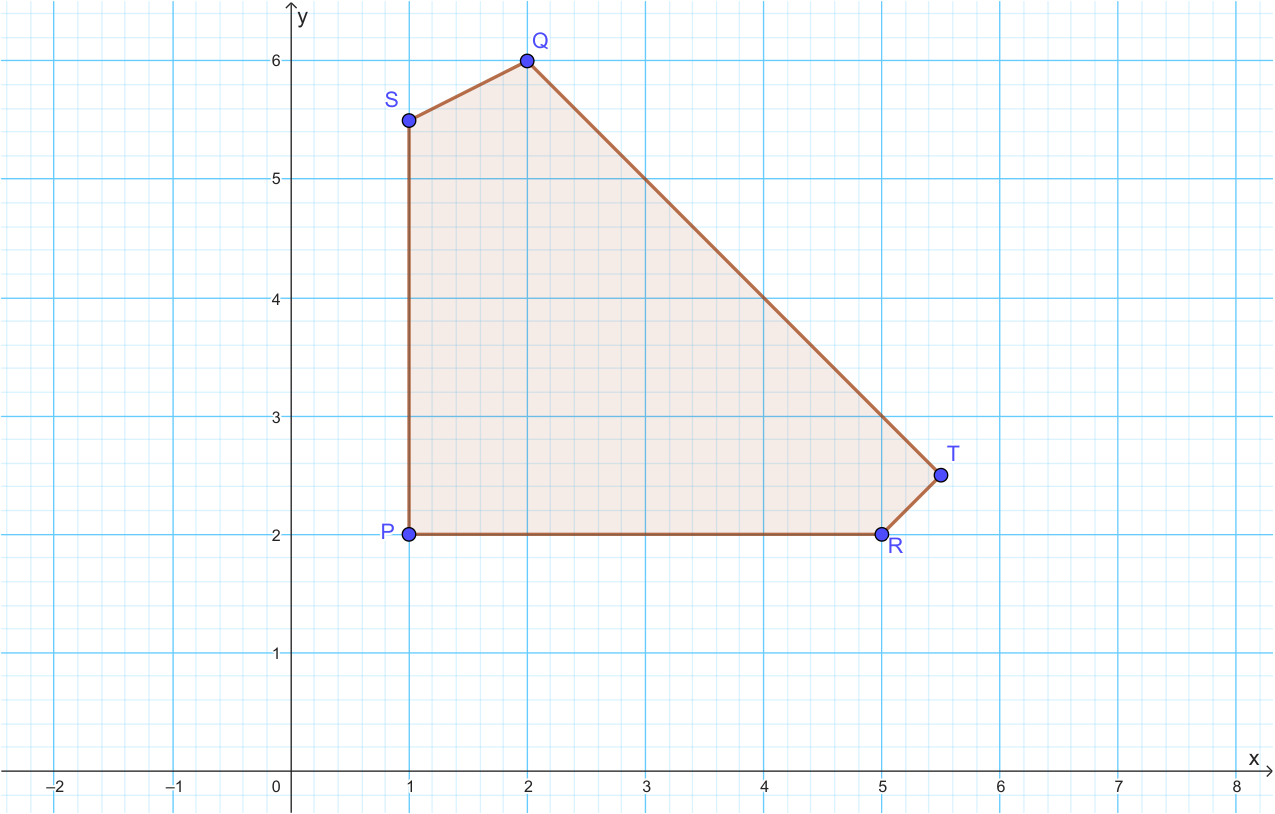
\includegraphics[width=0.85\linewidth]{figures/fig2-4.png}
\end{center}
\figcaption{2.4}{Graphical representation of inequalities in Example 2.15}

\textbf{Step 2:} Identify the coordinates of the vertices polygon created as a result of the
intersection of the lines.

P$(1, 2)$, S$(1, 5.5)$, Q$(2, 6)$, T$(5.5, 2.5)$ and R$(5, 2)$

\textbf{Step 3:} Substitute the values of the coordinates in the function $w = x^2 + y^2$.

For $(1, 2)$, $x = 1$, $y = 2$.
\begin{align*}
  w &= (1)^2 + (2)^2 \\
    &= 5
\end{align*}
For $(1, 5.5)$, $x = 1$, $y = 5.5$.
\begin{align*}
  w &= (1)^2 + (5.5)^2 \\
    &= 31.25
\end{align*}
For $(2, 6)$, $x = 2$, $y = 6$.
\begin{align*}
  m &= (2)^2 + (6)^2 \\
    &= 40
\end{align*}
For $(5.5, 2,5)$, $x = 5.5$, $y = 2.5$.
\begin{align*}
  m &= (5.5)^2 + (2.5)^2 \\
    &= 36.5
\end{align*}
For $(5, 2)$, $x = 5$, $y = 2$.
\begin{align*}
  m &= (5)^2 + (2)^2 \\
    &= 29
\end{align*}

\textbf{Step 4:} Select the highest result as the maximum value and the least as the
minimum value

Maximum value is 40 at vertex $(2, 6)$.

Minimum value is 5 at vertex $(1, 2)$.
\booknote{the last three substitutions are printed with ``$m =$'' in the book although
the function is $w$; ``$(5.5, 2,5)$'' is also as printed.}
\end{example}

Now, let's see how our knowledge on solving linear inequalities can be used to
solve real life problems.
